% !TEX encoding = UTF-8
% !TEX program = pdflatex
% !TEX root = MEMOC.tex
% !TEX spellcheck = it-IT

\chapter{Laboratorio}

\section{Introduzione}

Come solver per i nostri modelli utilizzeremo CPLEX.

Un solver è un'applicazione che prende in input la descrizione di un modello relativo ad un problema di ottimizzazione e fornisce in output una soluzione ottima del problema.

\begin{figure}[htbp]
	\centering
	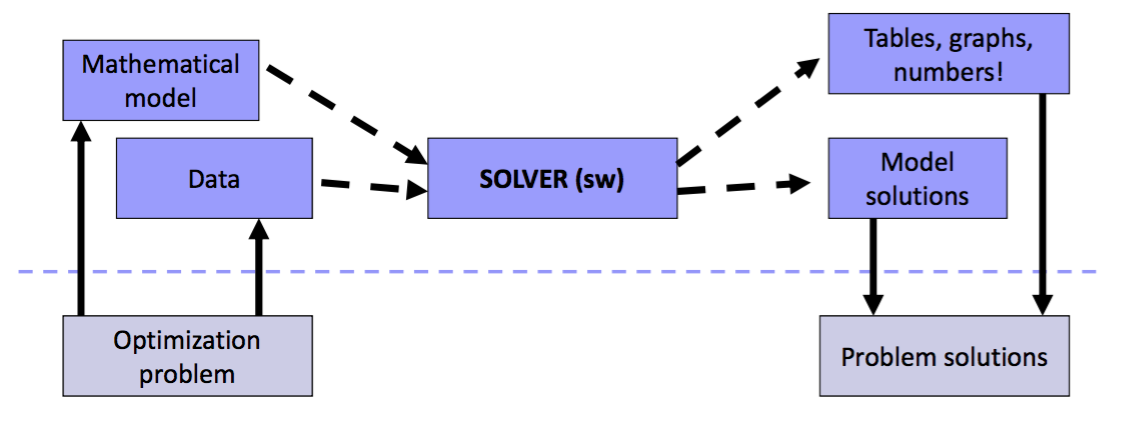
\includegraphics[width=0.7\linewidth]{./images/lab1-schema-1}
\end{figure}

Ovviamente il modello deve essere espresso in una particolare sintassi.

CPLEX è un solver MILP, ovvero un solver in grado di risolvere problemi di programmazione lineare intera mista.
Questa tipologia di solver è quella più comune perché è molto efficiente, non soffre di problemi legati alla stabilità numerica e risulta facilmente embeddabile in altri programmi.

Come anticipato, ogni solver ha una sua interfaccia che può essere utilizzata da dei linguaggi special-purpose o general-purpose.

\begin{figure}[htbp]
	\centering
	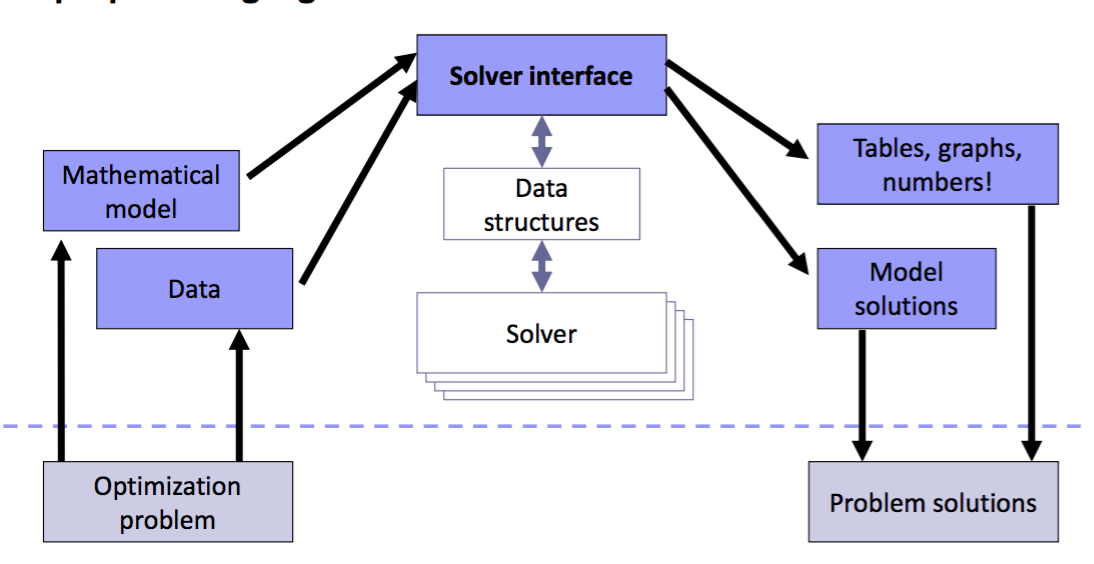
\includegraphics[width=0.7\linewidth]{./images/lab1-schema-2}
\end{figure}

\section{Introduzione a CPLEX}

CPLEX è stato uno dei primi solver e al momento è tra i migliori, in quanto include lo stato dell'arte delle varie tecnologie.

Ci sono varie interfacce utilizzabili per i vari linguaggi di programmazione più diffusi e anche per i linguaggi special-purpose come AMPL. Noi utilizzeremo le API C/C++.

Le \textbf{CPLEX Callable Libraries} implementano varie algoritmi di risoluzione, noi utilizzeremo il MIP, e sono composte da due oggetti principali: \texttt{Environment} e \texttt{Problem}.

\begin{itemize}
	\item \texttt{Enviroment}: contiene le informazioni relative ai parametri di ottimizzazione, alla configurazione, ecc.
	\item \texttt{Problem}: contiene le informazioni di un particolare problema, come i vincoli e le variabili.
\end{itemize}

\noindent\`E necessario che venga definito almeno un \texttt{Environment} e un \texttt{Problem}.

\begin{verbatim}
CPXENVptr CPXopenCPLEX / CPLcloseCPLEX
CPXLPptr CPLcreateprob / CPXfreeprob
\end{verbatim}

\noindent Per interagire con gli oggetti vengono usate le apposite API che seguono più o meno lo stesso schema

\begin{verbatim}
int CPXfuncName (eviroment[,problem],...);
\end{verbatim}

\noindent L'intero ritornato è un codice errore, se è 0 vuol dire che l'operazione è andata a buon fine.

\section{Rappresentazione con matrici sparse}

Un modello generico può essere rappresentato da delle matrici:

\begin{align*}
\min/\max & C^T x \\
\st & A x = b \\
	& x \geq 0
\end{align*}

\noindent con $x,C \in \mathbb{R}^n$, $A \in \mathbb{R}^{m \times n}$ e $b \in \mathbb{R}^m$.

Nei casi reali la matrice $A$ risulta essere molto grande e sparsa, ovvero con molti elementi uguali a 0.

Questa matrice viene quindi rappresentata con 3 vettori:

\begin{itemize}
	\item \texttt{double* val}: contiene i valori della matrice in modo compatto (uno dietro l'altro).
	\item \texttt{int* idx}: contiene l'indice della colonna del valore che si trova alla stessa posizione del vettore \texttt{val}. La lunghezza di \texttt{idx} è la stessa di \texttt{val}.
	\item \texttt{int* beg}: contiene gli indici per il vettore \texttt{val} dove iniziano le righe della matrice.
\end{itemize}

\begin{figure}[htbp]
	\centering
	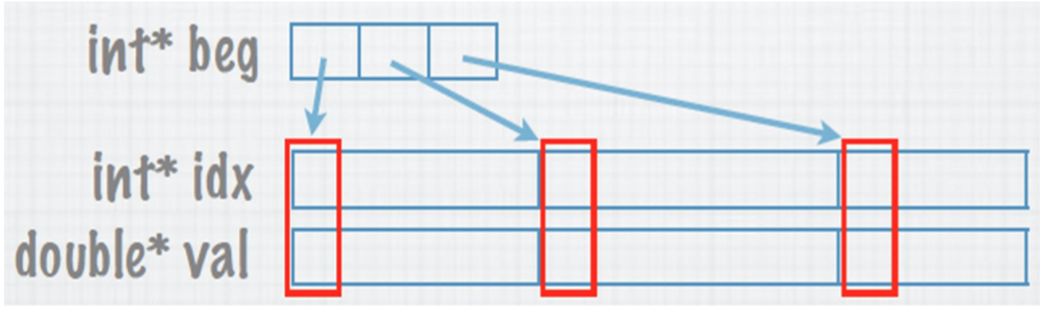
\includegraphics[width=0.5\linewidth]{./images/lab1-matrix}
\end{figure}

\section{Utilizzo di CPLEX}

Per avviare l'ambienti di CPLEX nel terminale è necessario eseguire i comandi:

\begin{verbatim}
$ . clpex_env
$ cplex
\end{verbatim}

\noindent Nel file \texttt{02.firstModel/cpxmacro.h} ci sono delle macro che facilitano la creazione dell'ambiente e del problema.
Abbiamo pure un Makefile che compila tutto, che bello!

Le macro a disposizione permetto di creare facilmente un ambiente e un problema CPLEX:

\begin{itemize}
	\item \texttt{DECL\_ENV(name)}: dichiara una variabile ambiente CPLEX di nome \texttt{name}.
	\item \texttt{DECL\_PROB(env, name)}: dichiara una variabile problema CPLEX di nome \texttt{name}. \texttt{env} rappresenta il contesto CPLEX del problema.
	\item \texttt{CHECKED\_CPX\_CALL(func, env, ...)}: invoca la funzione \texttt{func} nell'ambiente \texttt{env}, passandole i vari parametri extra. Questa macro implementa un controllo sul valore di ritorno della funzione per verificare l'assenza di errori.
\end{itemize}

\subsection{Definizione delle variabili}

Le variabili di un problema CPLEX vengono anche dette colonne perché nella rappresentazione con la matrice sparsa vengono associate alle colonne della matrice.

Per dichiarare nuove variabili la funzione CPLEX da invocare è

\begin{center}
\texttt{CPXnewcols (env, lp, ccnt, obj, lb, ub, xctype, colname);}
\end{center}

\begin{itemize}
	\item \texttt{env}: l'ambiente CPLEX;
	\item \texttt{lp}: il problema;
	\item \texttt{ccnt}: il numero di variabili da aggiungere al problema;
	\item \texttt{obj}: i coefficienti delle variabili all'interno della funzione obiettivo;
	\item \texttt{lb/ub}: i lower bound e upper bound del dominio delle variabili;
	\item \texttt{xctype}: i tipi delle variabili:
	\begin{itemize}
		\item \texttt{'C'}: variabile continua (reale);
		\item \texttt{'B'}: variabile binaria;
		\item \texttt{'I'}: variabile intera.
	\end{itemize}
	\item \texttt{colname}: nomi delle variabili. Se viene passato \texttt{NULL}, CPLEX assegnerà dei nomi di default.
\end{itemize}

\noindent Da notare che tutti i parametri che descrivono le variabili sono degli array, pertanto è importante che gli elementi degli array siano sempre \textbf{nello stesso ordine}, ovvero in tutti gli array il primo elemento descrive la prima variabile che viene inserita, tutti i secondi elementi descrivono la seconda e così via.

Esempio di chiamata utilizzando le macro:

\begin{lstlisting}[language=C++]
// Vettore con i costi nella funzione obiettivo
double objCost[6] = {    2.0, 3.0, 0.0, 0.0, 0.0, 1.0 };
// variable lower and upper bounds
// Anche in questo caso l'ordine e' importante
double lb[6]      = {    0.0         , 0.0 , -CPX_INFBOUND , -CPX_INFBOUND , 0 , 0};
double ub[6]      = { CPX_INFBOUND, CPX_INFBOUND , 0 , CPX_INFBOUND , 1 , CPX_INFBOUND};
// variable types 'C' or 'B' or 'I' ...
// C -> Continuos? Real
// B -> Binary
// I -> Integer
char xtype[6]     =  { 'C', 'C', 'C', 'C', 'B', 'I' };

// Nomi delle variabili
char ** xname = NULL;

// CPXnewcols e' la funzione da invocare
CHECKED_CPX_CALL( CPXnewcols, env, lp, 6, &objCost[0], &lb[0], &ub[0], &xtype[0], xname );
\end{lstlisting}

\subsection{Definizione dei vincoli}

I vincoli di un problema CPLEX vengono anche detti righe perché nella rappresentazione con la matrice sparsa vengono associate alle righe della matrice.

Per dichiarare dei nuovi vincoli la funzione CPLEX da invocare è

\begin{center}
\texttt{CPXaddrows (env, lp, colcnt, rowcnt, nzcnt, rhs, sense, rmatbeg, rmatind, rmatval , newcolname, newrowname);}
\end{center}

\begin{itemize}
	\item \texttt{colcnt}: numero di colonne (variabili) da creare. Posso anche essere aggiunte delle variabili in contemporanea ai vincoli, ma è sconsigliato. Per evitare di aggiungere nuove variabili basta passare 0.
	\item \texttt{rowcnt}: numero di vincoli da aggiungere.
	\item \texttt{nzcnt}: numero di coefficienti della matrice sparsa che sono diversi da 0.
	\item \texttt{rhs}: parametro \texttt{b} del modello, ovvero il vettore con i valori presenti nella parte destra dei vincoli.
	\item \texttt{sense}: senso dei vincoli: \texttt{'G'} ($\geq$), \texttt{'E'} ($=$), \texttt{'L'} ($\leq$).
	\item \texttt{rmatbeg}: vettore con gli inizi delle righe della matrice sparsa (\textit{beg}).
	\item \texttt{rmatind}: vettore con gli indici di riga della matrice sparsa (\textit{idx}).
	\item \texttt{rmatval}: vettore con i valori della matrice sparsa.
	\item \texttt{newcolname/newrowname}: nomi per le colonne/righe. 
\end{itemize}

\noindent Anche in questo caso, l'ordine degli elementi all'interno dei vettori è importante.

Esempio di chiamata utilizzando le macro:

\begin{lstlisting}[language=C++]
int colcount = 0;

int rowcount = 4;

// NB: se una variabile compare nella parte destra, deve comunque finire nella
//     matrice dei coefficienti, con il coefficiente di segno opposto.
int nzcnt = 11;

// right-hand-sides: i vincoli sono stati riscritti in modo che nella parte destra non compaiano variabili
double rhs[4] = { 0.0, 2, -1, 9 };

// Tipo di vincolo: 'L', 'E', 'G'
char sense[4] = {'L','E', 'G', 'L'};

// the coefficient matrix will be linearized in a vector and ONLY NON-ZERO coefficients
//  need to be stored: the following three vectors are used
// the linearized vector of non-zero coefficients
// anche in questo caso l'ordine dei vincoli e' importante
double rmatval[11] = { 1.0, 1.0, -5.0,   1.0, 9.0, 9.0, 8.0,     8.0,      -4.0, 7.0, 5.0 };

// one element for each constraint (row), reporting the index where each row of the coefficient matrix starts
int rmatbeg[4]    = { 0 , 3, 7, 8};

// one element for each zon-zero ceofficient, reporting its column index 
//                      x1   x2   z 
int rmatind[11]    = {  0  , 1  , 4,
//                      x2  y1  y2  w
                        1 , 2 , 3 , 5,
//                      y1
                        2 ,
//                      y1  z   w
                        2 , 4 , 5
};

char ** newcolnames = NULL;
char ** rownames = NULL;

CHECKED_CPX_CALL( CPXaddrows, env, lp, colcount, rowcount, nzcnt, &rhs[0], &sense[0], &rmatbeg[0], &rmatind[0], &rmatval[0], newcolnames , rownames );
\end{lstlisting}

\subsection{Risoluzione del problema}

Come prima cosa è necessario specificare se si tratta di un problema di massimizzazione o di minimizzazione, utilizzando la funzione \texttt{CPXchobjsen}. Di default il problema è una minimizzazione.

Dopodiché per risolvere il problema è necessario specificare quale algoritmo utilizzare. Nel corso noi useremo sempre l'algoritmo MIP.

\begin{lstlisting}[language=C++]
// configura la massimizzazione
// MAXimize o MINimize
CHECKED_CPX_CALL( CPXchgobjsen, env, lp, CPX_MAX );

// Stampa il modello su un file, utile per effettuare il debug
CHECKED_CPX_CALL( CPXwriteprob, env, lp, "primo.lp", NULL );

// risolve con l'algoritmo MIP
CHECKED_CPX_CALL( CPXmipopt, env, lp );
\end{lstlisting}
